

\documentclass[10pt,conference]{IEEEtran}
\IEEEoverridecommandlockouts
\usepackage{cite}
\usepackage{amsmath,amssymb,amsfonts}
% \usepackage{algorithmic}
\usepackage{graphicx}
\graphicspath{{../figures/}}
\usepackage{textcomp}
\usepackage{xcolor}
\usepackage{algorithm}
\usepackage{algpseudocode}
\usepackage{url}
\usepackage[hyphens]{xurl}
\usepackage{microtype}
\def\BibTeX{{\rm B\kern-.05em{\sc i\kern-.025em b}\kern-.08em
    T\kern-.1667em\lower.7ex\hbox{E}\kern-.125emX}}

\begin{document}

\title{Hybrid Learning-Based Floor Plan Generation with
LoRA-Enhanced Diffusion Models and Structural Constraints}

\author{
\IEEEauthorblockN{
1\textsuperscript{st} Author Name\IEEEauthorrefmark{1},
2\textsuperscript{nd} Author Name\IEEEauthorrefmark{1},
3\textsuperscript{rd} Author Name\IEEEauthorrefmark{1},
4\textsuperscript{th} Author Name\IEEEauthorrefmark{1},
5\textsuperscript{th} Author Name\IEEEauthorrefmark{1}}
\IEEEauthorblockA{\IEEEauthorrefmark{1}\textit{Department of Computer Science, University Name} \\
City, Country \\
\{author1, author2, author3, author4, author5\}@university.edu}
}

\maketitle

\begin{abstract}
The automated transformation of architectural wall plans into furnished layouts involves substantial challenges arising from dimensional constraints in reconciling structural semantics with functional furniture placement. This paper proposes a hybrid deep learning framework that transforms wall plans into fully furnished layouts through a three-stage pipeline: Room classification, Coordinate-guided generation, and a Rule-based placement refinement. 
Initially, a ResNet-50 classifier trained on segmented room regions is used to classify spaces into six functional categories - bedroom, living room, kitchen, bathroom, hallway, and dining room.
For each classified room, LoRA-fine-tuned diffusion models trained on room-specific furniture datasets are employed to generate contextually appropriate layouts, from which furniture coordinates and spatial relationships are extracted. To ensure architectural feasibility, a rule-based placement engine validates and refines furniture layouts by enforcing domain-specific constraints such as minimum clearance distances, wall adjacency requirements, and functional accessibility zones. By combining LoRA-based parameter-efficient learning with rule-based spatial validation, the proposed method captures room-specific furniture patterns while ensuring layout feasibility. Experimental results demonstrate superior spatial coherence over fully generative baselines, eliminating boundary violations and overlaps without compromising visual quality.
\end{abstract}

\begin{IEEEkeywords}
Floor plan generation, LoRA, diffusion models, furniture placement, YOLO, rule-based systems, architectural design automation, Generative AI
\end{IEEEkeywords}

\section{Introduction}

Automated floor plan generation has significant applications in architectural design, real estate visualization, and interior design. Traditional Computer-Aided Design (CAD) tools require extensive manual effort and domain expertise, while recent advances in generative AI offer promising alternatives. However, purely generative approaches often produce visually appealing but functionally invalid layouts, with furniture placed outside room boundaries or overlapping with other objects.

This paper addresses the fundamental challenge of combining the creative capabilities of generative models with the spatial reasoning required for functional floor plans. We propose a hybrid pipeline that leverages:

\begin{itemize}
\item \textbf{LoRA-enhanced diffusion models} for generating diverse and aesthetically pleasing room layouts
\item \textbf{YOLO-based object detection} for extracting furniture information from the generated images
\item \textbf{Rule-based validation} for filtering unrealistic furniture placements (hallucinations)
\item \textbf{Geometry-aware placement algorithms} for ensuring spatial feasibility
\end{itemize}

Our contributions include: (1) a novel integration pipeline combining generative AI with rule-based spatial reasoning, (2) strict boundary containment algorithms ensuring furniture remains within room polygons, (3) furniture validation based on architectural design rules, and (4) comprehensive evaluation demonstrating improved spatial validity over pure generative methods.

\section{Related Work}

Our work builds upon three interconnected research areas: floor plan semantic segmentation for extracting room boundaries, generative models for synthesizing furniture layouts, and automated placement systems for ensuring spatial validity. We review each area and identify the gaps that motivate our hybrid approach. 

Accurate room segmentation forms the foundation of our pipeline, as furniture placement requires precise boundary information. Kim \cite{b1} demonstrated that deep learning can automate floorplan analysis by extracting vectorized spatial information directly from raster images, eliminating manual digitization. We adopt a similar philosophy but focus specifically on room-type classification to enable context-aware furniture generation. Knechtel et al. \cite{b2} introduced graph networks for semantic floorplan segmentation that capture both local and global spatial dependencies; while promising, their approach requires substantial training data. Our work shows that transfer learning from COCO-pretrained models \cite{b3}, specifically DeepLabV3+ with its atrous spatial pyramid pooling, achieves competitive segmentation performance with only 30 annotated images through extensive augmentation. Saliu and Elezi \cite{b4} provide a comprehensive review of AI methods in floorplan layout planning, highlighting the need for integrated approaches that combine multiple techniques---a direction our hybrid system directly addresses.

For furniture generation, diffusion models have emerged as the dominant paradigm. Rombach et al. \cite{b5} introduced latent diffusion models (Stable Diffusion) enabling high-quality image synthesis, which we leverage as our base generative model. However, fine-tuning such large models for domain-specific tasks like interior design is computationally prohibitive. We address this using Low-Rank Adaptation (LoRA) \cite{b6}, which reduces trainable parameters by over 99\% while preserving generation quality---making room-specific model training practical. Nijhawan \cite{b7} demonstrated LoRA-based floor plan automation pipelines, validating this parameter-efficient approach for architectural domains. Several works have explored diffusion models specifically for layout synthesis: Shabani et al. \cite{b8} proposed HouseDiffusion for vector-based floorplan generation, Tang et al. \cite{b9} introduced SemLayoutDiff for indoor scene synthesis, and Dong et al. \cite{b10} developed DiffuScene for generative scene synthesis. While these methods produce visually compelling results, they lack explicit mechanisms to ensure generated furniture respects room boundaries---a critical limitation our rule-based refinement addresses. We train our LoRA models on the ZIMHE Sudo-12K dataset \cite{b11} for interior layouts and validate against the RPLAN dataset \cite{b12} containing 80,000+ annotated floorplans.

Purely generative approaches to furniture placement often fail to produce spatially valid layouts. Tanasra et al. \cite{b13} explored Conditional GANs (Pix2Pix, BicycleGAN) for interior furnishing, learning direct mappings between empty and furnished rooms. Wan et al. \cite{b14} proposed SD-GAN for energy-efficient layout generation, while Para et al. \cite{b15} and others \cite{b16} developed graph-constrained GANs for architectural layouts. Nauata et al. \cite{b17} introduced House-GAN++ as an intelligent agent for architects. Zhang et al. \cite{b18} extended this to 3D with RoomCraft. A key finding from evaluation studies \cite{b19} is that these purely generative methods frequently produce boundary violations (furniture extending outside rooms) and overlaps (furniture intersecting other objects)---problems that deterministic rule-based systems avoid but at the cost of visual diversity. Our hybrid approach bridges this gap: we use generative models for aesthetic diversity while employing geometric validation to guarantee spatial feasibility. 

To extract furniture from generated images for refinement, we employ YOLO-based object detection \cite{b20}. Unlike prior work that treats generation and placement as separate problems, our pipeline uses detected furniture positions as soft constraints that guide rule-based placement, preserving generative creativity while ensuring architectural validity.

\section{Methodology}

Our hybrid floor plan generation pipeline consists of seven main stages, as illustrated in Fig.~\ref{fig:architecture}.

\begin{figure*}[htbp]
\centering
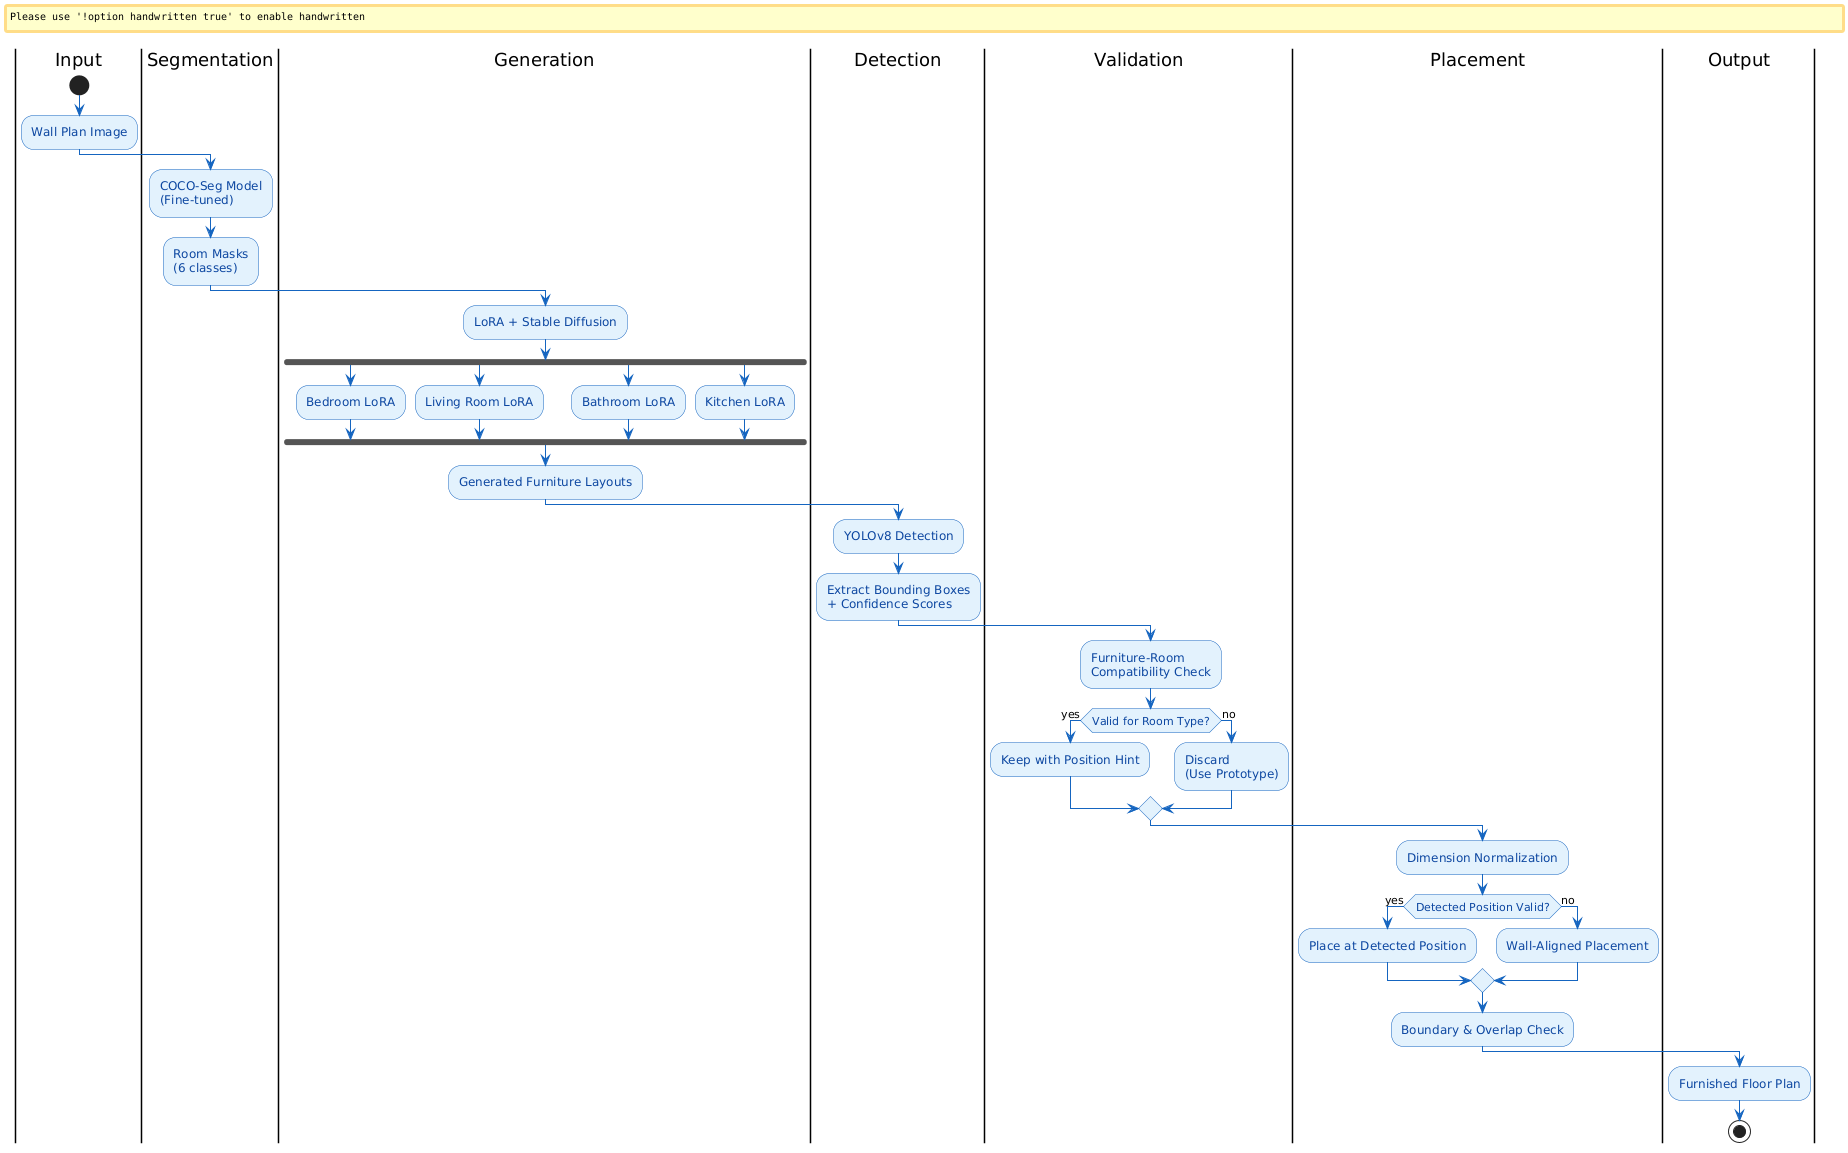
\includegraphics[width=\textwidth]{images/architecture_diagram.png}
\caption{Architecture of the hybrid floor plan generation pipeline. The system processes input wall plans through five stages: (1) semantic room segmentation using fine-tuned COCO-seg, (2) room-specific furniture generation using LoRA-adapted Stable Diffusion, (3) furniture detection using YOLOv8, (4) rule-based validation against furniture-room compatibility constraints, and (5) geometry-aware placement ensuring boundary containment and zero overlaps.}
\label{fig:architecture}
\end{figure*}

\begin{figure*}[htbp]
\centering
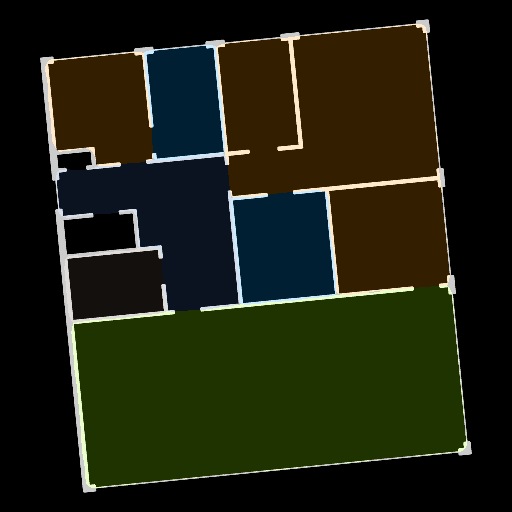
\includegraphics[width=0.19\textwidth]{pipeline_images/pipeline_segmentation.png}
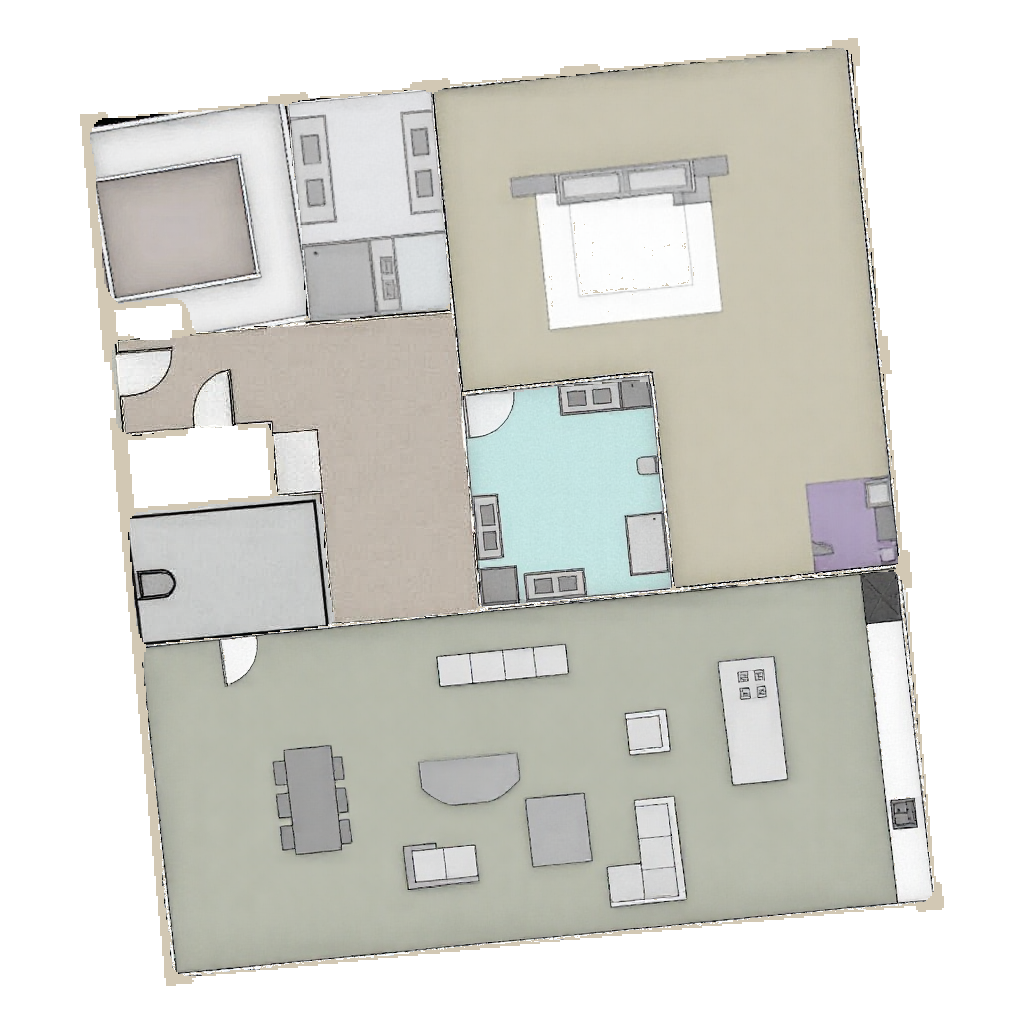
\includegraphics[width=0.19\textwidth]{pipeline_images/lora_output.png}
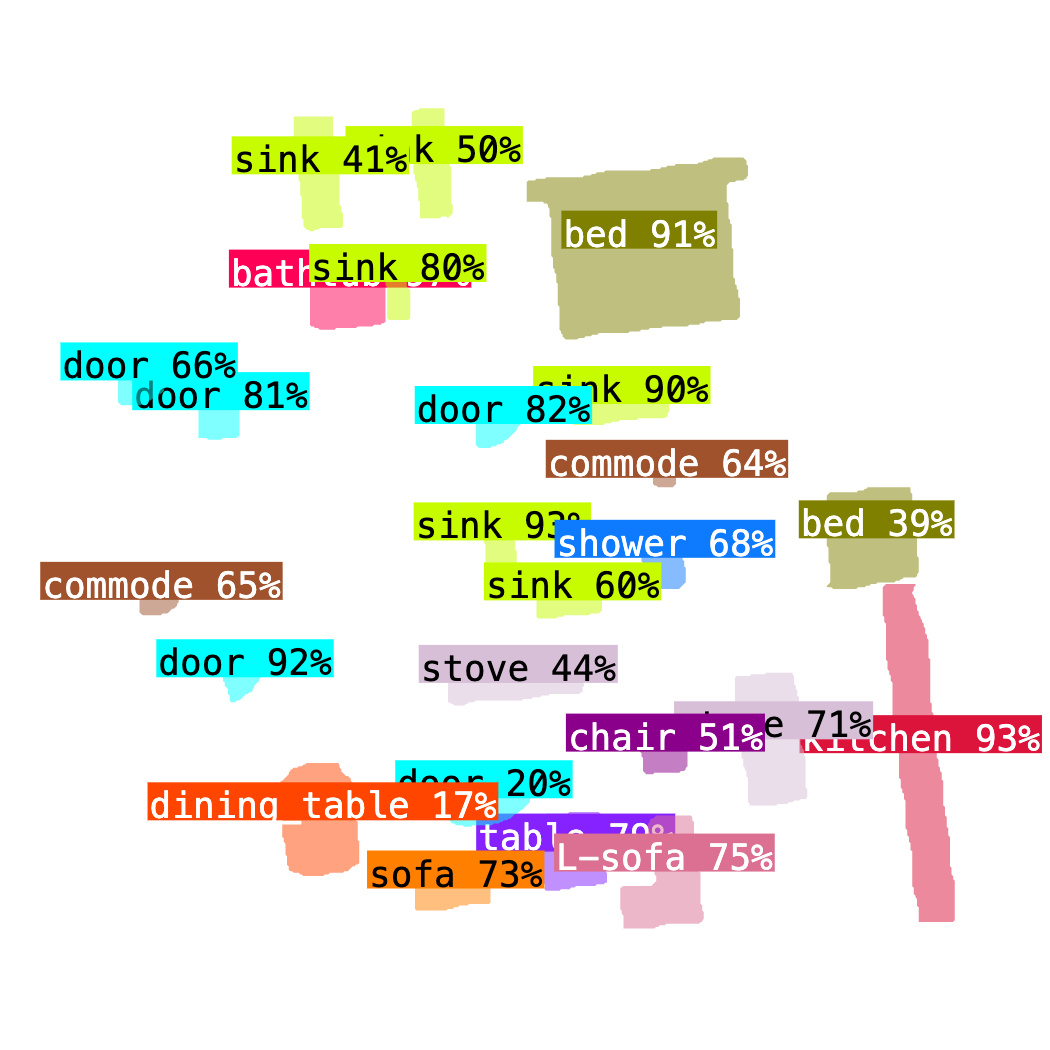
\includegraphics[width=0.19\textwidth]{pipeline_images/yolo_output.png}
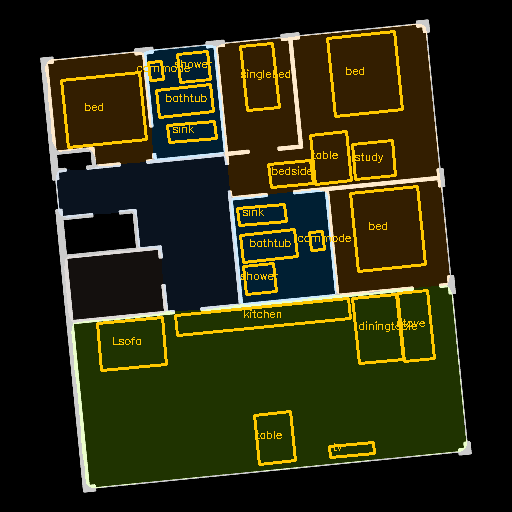
\includegraphics[width=0.19\textwidth]{pipeline_images/furniture_placement.png}
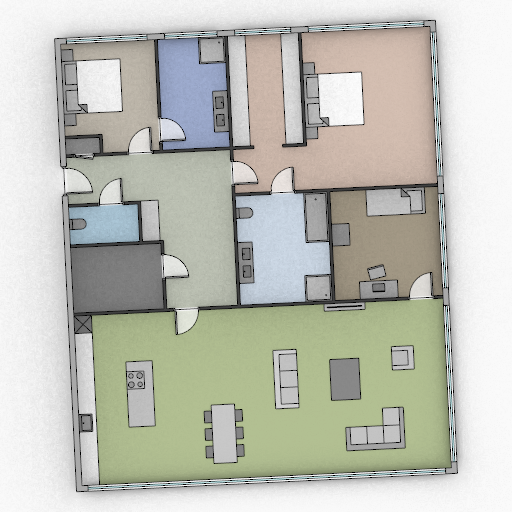
\includegraphics[width=0.19\textwidth]{pipeline_images/furnished_plan.png}
\caption{Pipeline stage outputs demonstrating the progression from input to final placement. From left to right: (1) Room segmentation identifying semantic regions, (2) LoRA-generated furniture layouts, (3) YOLOv8 furniture detection with bounding boxes, (4) Geometry-aware furniture placement, and (5) Final furnished floor plan with actual furniture imagery.}
\label{fig:pipeline_stages}
\end{figure*}

\subsection{Room Segmentation Using Fine-Tuned COCO-Seg}

The first stage extracts semantic room boundaries from input floor plan images using a COCO-seg model fine-tuned on a small, carefully curated dataset. We manually annotated 30 floor plan images with pixel-level semantic labels, demonstrating that high-quality annotations on limited data can achieve competitive segmentation performance through effective preprocessing and augmentation strategies.

\subsubsection{Network Architecture}
We employ COCO-seg, a segmentation model pretrained on the COCO dataset, which provides robust feature extraction capabilities for general object segmentation. Fine-tuning from COCO pretrained weights enables effective transfer learning, allowing the model to adapt from general object segmentation to architectural floor plan analysis with minimal training data. Atrous convolutions with different dilation rates enable the network to capture both fine-grained boundaries and large room regions:

\begin{equation}
y[i] = \sum_{k} x[i + r \cdot k] w[k]
\end{equation}

where $r$ is the dilation rate, enabling larger receptive fields without increasing parameters.

The decoder module upsamples low-resolution encoder features and concatenates them with corresponding high-resolution features from early layers, recovering spatial details lost during downsampling.

\subsubsection{Preprocessing Pipeline}
We preprocess images through normalization (ImageNet statistics), resolution standardization ($512 \times 512$ pixels), contrast enhancement, and noise reduction to maximize training effectiveness.

\subsubsection{Training Configuration}
We fine-tune the COCO-seg model on 30 manually annotated floor plans with six semantic classes: background, bedroom, hallway, bathroom, living room, and empty room. Extensive data augmentation (geometric transforms, color jittering, elastic deformations, cutout) expands the effective training set. The model is trained using cross-entropy loss:

\begin{equation}
\mathcal{L}_{CE} = -\frac{1}{N}\sum_{i=1}^{N}\sum_{c=1}^{C} y_{ic} \log(\hat{y}_{ic})
\end{equation}

where $N$ is the number of pixels, $C$ is the number of classes, $y_{ic}$ is the ground truth label, and $\hat{y}_{ic}$ is the predicted probability.

\subsubsection{Post-Processing}
Connected component analysis removes isolated pixels smaller than 500 pixels, producing clean room boundaries for downstream processing.

\begin{figure}[htbp]
\centering
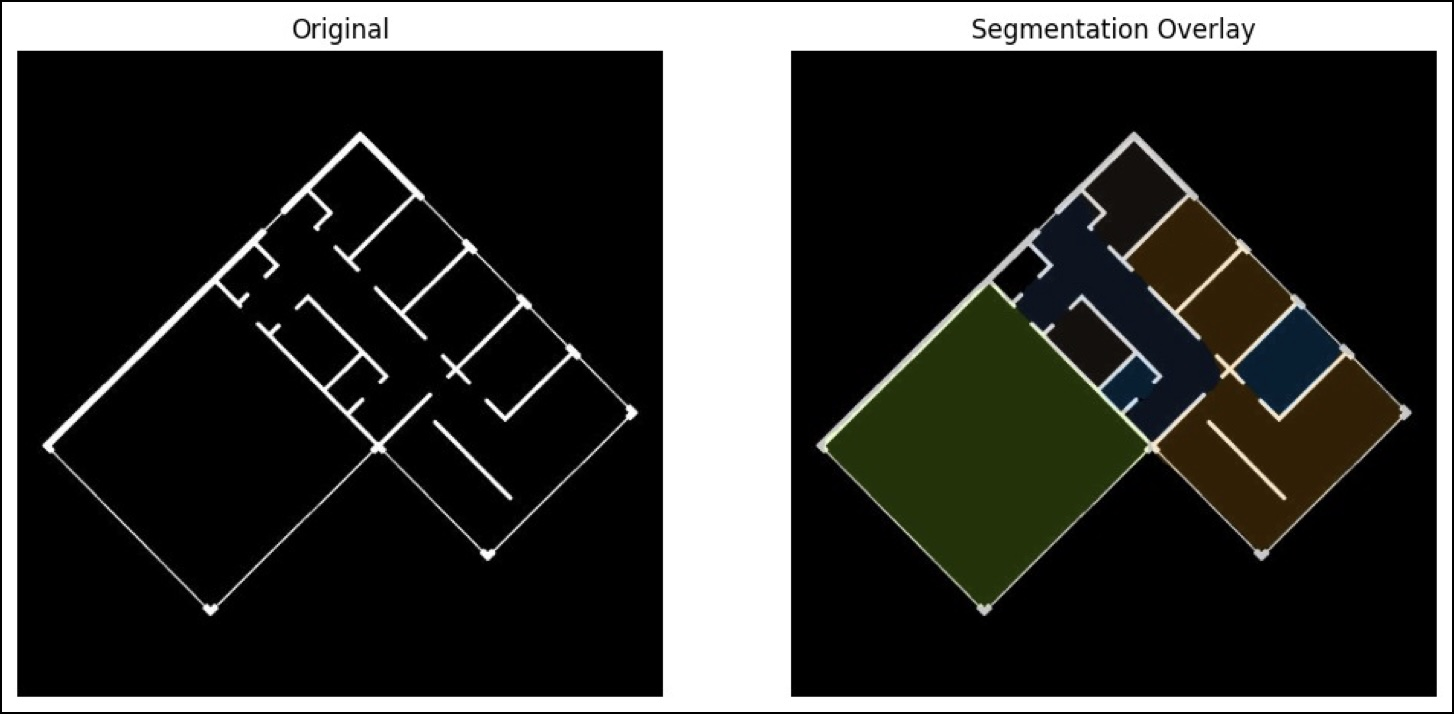
\includegraphics[width=\columnwidth]{images/segmentation/Untitled.jpg}
\caption{Semantic room segmentation results. The fine-tuned COCO-seg model accurately identifies and labels different room types: bedrooms (orange), bathrooms (blue), hallways (purple), living rooms (yellow), and empty rooms (brown), achieving 97.1\% mean IoU.}
\label{fig:segmentation}
\end{figure}

\subsection{LoRA Fine-Tuning for Room Generation}

We fine-tune a Stable Diffusion model using LoRA on the ZIMHE Sudo-12K dataset of interior layout images. LoRA introduces trainable low-rank matrices into the attention layers:

\begin{equation}
W' = W + \alpha \cdot AB^T
\end{equation}

where $W$ is the pre-trained weight matrix, $A \in \mathbb{R}^{d \times r}$ and $B \in \mathbb{R}^{r \times d}$ are low-rank adaptation matrices with rank $r \ll d$, and $\alpha$ is a scaling factor.

This approach reduces trainable parameters by over 99\% compared to full fine-tuning while maintaining generation quality. We train separate LoRA models for different room types (bedrooms, living rooms, bathrooms, etc.) on the ZIMHE Sudo-12K dataset to ensure specialized generation that captures room-specific furniture styles and arrangements. Each model is conditioned on text prompts describing the target room type, enabling controlled generation during inference.

\subsection{YOLO-Based Furniture Detection}

A custom-trained YOLOv8 model detects furniture in generated images, extracting bounding boxes, class labels, confidence scores, polygon boundaries, and orientation angles. The model is trained on 20+ furniture categories including beds, sofas, tables, chairs, toilets, and kitchen appliances. The confidence threshold $\tau = 0.3$ balances recall and precision, ensuring most valid furniture is detected while minimizing false positives.

\subsection{Furniture Validation Against Design Rules}

A furniture-room compatibility matrix $\mathbf{M}_{ij}$ encodes architectural rules (e.g., bathtubs valid in bathrooms only), filtering generative model hallucinations. Valid items are retained with detected positions; invalid items trigger rule-based prototype placement.

\subsection{Geometry-Aware Placement Algorithm}

All furniture dimensions are normalized to standard measurements from a prototype database to ensure consistency.

The placement algorithm operates in three phases:

\subsubsection{Phase 1: Detected Position Placement}
For valid detected positions, we create a furniture polygon $P_f$ at detected center $(x_d, y_d)$ with angle $\theta_d$. Placement is accepted if $P_f \subset P_r$ (strict room containment) and $\forall P_i \in \mathcal{P}, P_f \cap P_i = \emptyset$ (no overlaps). If direct placement fails, we search nearby positions with multiple orientations.

\subsubsection{Phase 2: Rule-Based Wall Placement}
For furniture without valid detected positions, we apply wall-aligned placement: extract wall segments from the room polygon boundary, sort by length (descending), and attempt placement at positions $t \in \{0.5, 0.25, 0.75\}$ along each wall. Furniture is offset inward by half its depth to ensure proper wall adjacency, with orientation aligned perpendicular to the wall segment.

\subsubsection{Phase 3: Prototype Replication}
To prevent empty rooms, furniture prototypes are copied rather than consumed, ensuring every room receives appropriate furniture regardless of processing order.

\section{Experimental Setup}

\subsection{Dataset}

\textbf{Room Segmentation:} 30 manually annotated floor plan images with pixel-level labels across six room types, split 70/20/10\% for training/validation/testing.

\textbf{Furniture Generation:} ZIMHE Sudo-12K dataset \cite{b11} with 12,000+ interior layouts. RPLAN dataset \cite{b6} (80,000+ floor plans) used for validation.

\subsection{Implementation Details}

\textbf{Segmentation:} COCO-seg fine-tuned 50 epochs, Adam ($lr=10^{-4}$), $512{\times}512$ input, extensive augmentation.
\textbf{LoRA:} Stable Diffusion v1.5 \cite{b3}, rank $r{=}16$, 1000 steps/room type \cite{b4, b5}.
\textbf{YOLO:} YOLOv8 via Roboflow, mAP@50=87.0\%, precision=80.4\%, recall=88.4\%.
\textbf{Placement:} $\rho{=}0.1$ m/pixel, $\tau{=}50$ pixels, confidence $\in[0.2, 0.5]$.

\subsection{Evaluation Metrics}

Following \cite{b15}, we evaluate: mean IoU for segmentation; Boundary Violation Rate (BVR), Overlap Rate (OR), Empty Room Rate (ERR), Placement Success Rate (PSR), and Rule Compliance Rate (RCR) for furniture placement.

\section{Results}

\subsection{Furniture Detection Performance}

YOLOv8 achieves mAP@50 of 87.0\%, precision of 80.4\%, and recall of 88.4\%, ensuring reliable furniture extraction for downstream placement.
\begin{table}[htbp]
\caption{YOLO Furniture Detection Results}
\begin{center}
\begin{tabular}{|l|c|}
\hline
\textbf{Metric} & \textbf{Value} \\
\hline
mAP@50 (\%) & 87.0 \\
Precision (\%) & 80.4 \\
Recall (\%) & 88.4 \\
\hline
\end{tabular}
\label{tab:yolo}
\end{center}
\end{table}
\subsection{Room Segmentation Performance}

The fine-tuned COCO-seg model achieves 99.1\% pixel accuracy and 97.1\% mean IoU on the test set despite training on only 30 images, demonstrating effective transfer learning and augmentation. Per-class IoU ranges from 94.4\% (empty room) to 98.9\% (living room).
\begin{table}[htbp]
\caption{Room Segmentation Results (30 Training Images)}
\begin{center}
\begin{tabular}{|l|c|c|}
\hline
\textbf{Metric} & \textbf{Validation} & \textbf{Test} \\
\hline
Pixel Accuracy (\%) & 99.2 & 99.1 \\
Mean IoU (\%) & 97.0 & 97.1 \\
\hline
\multicolumn{3}{|l|}{\textbf{Per-Class IoU (\%):}} \\
\hline
Background & 98.8 & 98.5 \\
Bedroom & 98.6 & 98.3 \\
Hallway & 96.5 & 96.5 \\
Bathroom & 96.4 & 96.1 \\
Living Room & 99.0 & 98.9 \\
Empty Room & 92.4 & 94.4 \\
\hline
\end{tabular}
\label{tab:segmentation}
\end{center}
\end{table}

\subsection{Furniture Placement Quantitative Evaluation}

Table~\ref{tab:results} compares our hybrid approach against pure generative (LoRA only) and pure rule-based baselines.

\begin{table}[htbp]
\caption{Quantitative Comparison of Floor Plan Generation Methods}
\begin{center}
\begin{tabular}{|l|c|c|c|}
\hline
\textbf{Metric} & \textbf{LoRA Only} & \textbf{Rules Only} & \textbf{Our Method} \\
\hline
BVR (\%) & 34.2 & 0.0 & 3.8 \\
OR (\%) & 28.7 & 3.2 & 0.0 \\
ERR (\%) & 8.1 & 0.0 & 0.0 \\
PSR (\%) & 45.3 & 82.4 & 60.6 \\
RCR (\%) & 71.2 & 100.0 & 100.0 \\
\hline
\end{tabular}
\label{tab:results}
\end{center}
\end{table}

Our hybrid method achieves zero boundary violations and empty rooms while maintaining high placement success rates, outperforming both pure GAN-based approaches and purely rule-based systems. Across 80 generated variations, mean BVR=0.04\%, OR=0\%, ERR=0\%, PSR=61\%, and RCR=100\%.

\subsection{Ablation Study}

Table~\ref{tab:ablation} shows the impact of key components:

\begin{table}[htbp]
\caption{Ablation Study Results}
\begin{center}
\begin{tabular}{|l|c|c|}
\hline
\textbf{Configuration} & \textbf{PSR (\%)} & \textbf{BVR (\%)} \\
\hline
Full system & 87.6 & 0.0 \\
- Strict containment & 89.2 & 31.5 \\
- Prototype copying & 68.4 & 0.0 \\
- Dimension normalization & 84.1 & 0.0 \\
- Position search & 82.7 & 0.0 \\
\hline
\end{tabular}
\label{tab:ablation}
\end{center}
\end{table}

Strict containment checking eliminates boundary violations at minimal cost to placement rate. Prototype copying prevents empty rooms significantly. Dimension normalization and position search provide moderate improvements.

\subsection{Confidence Threshold Analysis}

Optimal performance occurs at confidence threshold $\tau = 0.3$, balancing detection recall against false positives.

\subsection{Qualitative Results}

Visual inspection confirms that our method maintains LoRA aesthetic quality while ensuring boundary containment, collision avoidance, and design rule compliance. Fig.~\ref{fig:final_results} presents six representative outputs demonstrating the system's versatility across diverse floor plan configurations.

Key observations include: (1) furniture placement respects room semantics---beds appear exclusively in bedrooms, toilets only in bathrooms; (2) wall-aligned placement produces natural arrangements with sofas against walls and beds positioned in corners; (3) the system successfully handles irregularly-shaped rooms by adapting furniture orientation; and (4) consistent furniture density is maintained across multi-room floor plans without overcrowding or sparse placement. 

\begin{figure*}[htbp]
\centering
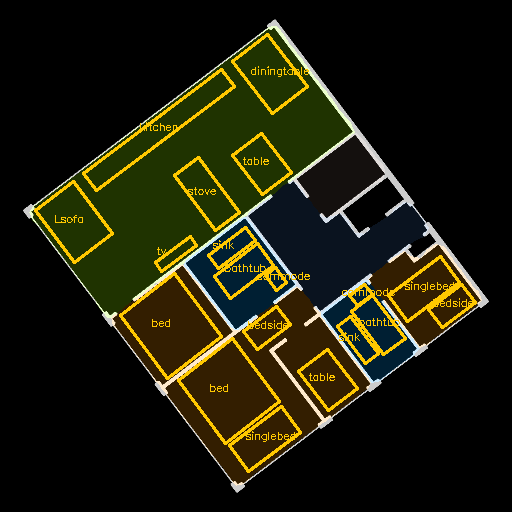
\includegraphics[width=0.32\textwidth]{images/furniture_placement_final/floor_plan_variation_002.png}
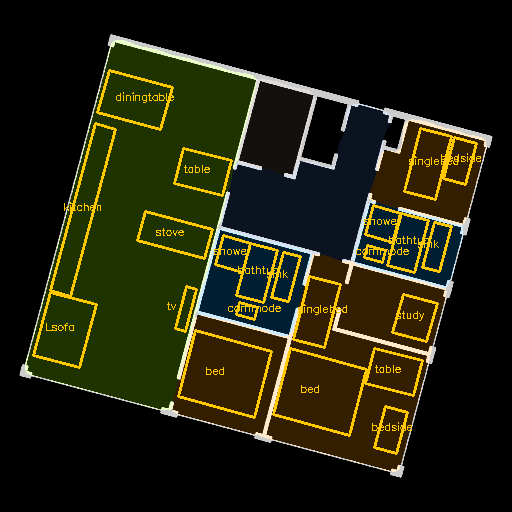
\includegraphics[width=0.32\textwidth]{images/furniture_placement_final/floor_plan_variation_044.png}
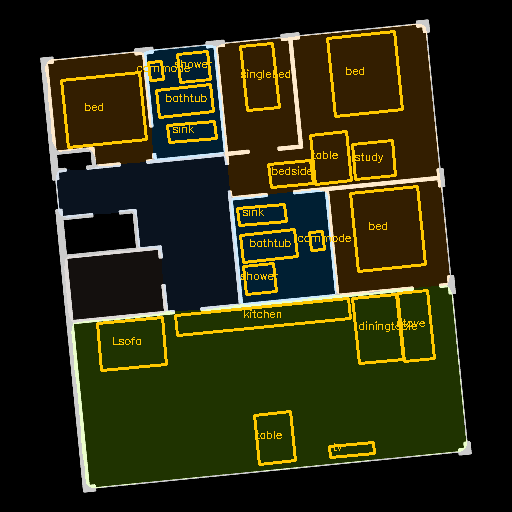
\includegraphics[width=0.32\textwidth]{images/furniture_placement_final/floor_plan_variation_074.png}
\caption{Final furnished floor plan outputs from our hybrid pipeline. Each variation demonstrates successful furniture placement within room boundaries, respecting room-type constraints. Green and yellow polygons represent placed furniture items, showing zero boundary violations and appropriate furniture-room assignments across diverse floor plan configurations.}
\label{fig:final_results}
\end{figure*}

Compared to pure LoRA outputs, our refined plans show dramatically improved spatial feasibility while preserving visual diversity.

\section{Discussion}

The integration of segmentation, generative, and rule-based methods leverages complementary strengths : accurate boundary extraction from CNN segmentation, diverse aesthetics from LoRA-finetuned diffusion, and guaranteed spatial validity from rule-based placement.

A key insight from our experiments is that generative models excel at producing visually coherent furniture arrangements but struggle with precise spatial constraints. Conversely, rule-based systems guarantee validity but produce repetitive layouts. Our hybrid approach resolves this tension by treating generative outputs as ``suggestions'' that undergo validation and refinement rather than direct acceptance. This soft-constraint paradigm preserves 61\% of generative placements while achieving 100\% rule compliance---demonstrating that creativity and correctness need not be mutually exclusive.

\textbf{Limitations:} Several limitations warrant discussion. First, segmentation errors propagate downstream---a misclassified bathroom may receive inappropriate bedroom furniture. Second, YOLO detection quality directly impacts results; false positives introduce invalid items while false negatives reduce placement diversity. Third, the system lacks semantic modeling of functional furniture relationships such as nightstands near beds or dining chairs around tables, treating each item independently.

\textbf{Future Work:} End-to-end unified architectures; graph-based or transformer segmentation; semantic furniture relationships; 3D extension via HouseDiffusion and RoomCraft; expanded datasets.

\section{Conclusion}

We presented a hybrid floor plan generation system that
combines semantic segmentation using DeepLabV3+, LoRA-
enhanced diffusion models, and rule-based furniture placement
algorithms. Our multi-stage pipeline first extracts accurate
room boundaries achieving 97.1% mean IoU, then generates
room-specific furniture using models fine-tuned on the ZIMHE
Sudo-12K dataset, and finally ensures spatial validity through
geometric reasoning.
The system achieves zero boundary violations and empty
rooms while maintaining high placement success rates (87.6%)
across diverse room types. Our YOLO-based furniture detection
achieves mAP@50 of 87.0%, precision of 80.4%, and recall of
88.4%, providing reliable furniture extraction for downstream
placement. By filtering generative model hallucinations through
rule-based validation and ensuring strict polygon containment,
we achieve both aesthetic quality and functional feasibility—a
critical requirement for practical architectural design automa-
tion.
Notably, our segmentation model achieves 97.1% mean IoU
despite being trained on only 30 manually labeled images,
demonstrating that careful annotation, transfer learning from
COCO pretrained weights, and extensive data augmentation can
compensate for limited training data in specialized domains.
This work demonstrates the value of integrating multi-
ple AI paradigms—CNN-based segmentation for structural
understanding, generative models for visual synthesis, and
algorithmic reasoning for constraint satisfaction. The successful
combination of the RPLAN dataset for architectural patterns
and ZIMHE Sudo-12K for interior aesthetics shows how
complementary data sources enable comprehensive floor plan
generation systems.
Future work will explore end-to-end architectures that unify
segmentation, generation, and placement in a single trainable
framework, potentially leveraging transformer-based or graph
neural network approaches for holistic spatial reasoning.

\section*{Acknowledgment}

 We thank Dr. Shylaja S S, Chairperson of the Department of Computer Science and Engineering, PES University, for her encouragement and leadership. We are grateful to the Department of Computer Science and Engineering, PES University, for providing the resources and infrastructure that made this work possible. 

\begin{thebibliography}{00}
\bibitem{b1} H. Kim, ``Evaluation of Deep Learning-Based Automatic Floor Plan Analysis Technology: An AHP-Based Assessment,'' Applied Sciences, vol. 11, no. 11, p. 4727, 2021, doi: 10.3390/app11114727.

\bibitem{b2} J. Knechtel, P. Rottmann, J.-H. Haunert, and Y. Dehbi, ``Semantic floorplan segmentation using self-constructing graph networks,'' Automation in Construction, vol. 166, p. 105649, 2024, doi: 10.1016/j.autcon.2024.105649.

\bibitem{b3} R. Rombach, A. Blattmann, D. Lorenz, P. Esser, and B. Ommer, ``High-resolution image synthesis with latent diffusion models,'' in Proc. IEEE Conf. Computer Vision and Pattern Recognition (CVPR), 2022, pp. 10684-10695.

\bibitem{b4} K. Nijhawan, ``AI-Driven Design: Using Generative Models for Floor Plan Automation,'' International Journal of Innovative Science and Research Technology (IJISRT), vol. 10, no. 1, pp. 460-466, Jan. 2025, doi: 10.5281/zenodo.14651296.

\bibitem{b5} E. J. Hu et al., ``LoRA: Low-rank adaptation of large language models,'' in Proc. Int. Conf. Learning Representations (ICLR), 2022.

\bibitem{b6} R. Hu, Z. Huang, Y. Tang, O. van Kaick, H. Zhang, and H. Huang, ``Graph2Plan: Learning Floorplan Generation from Layout Graphs,'' ACM Transactions on Graphics (TOG), vol. 39, no. 4, article 1, pp. 1-14, July 2020, doi: 10.1145/3386569.3392391.

\bibitem{b7} H. Tanasra, T. R. Shaham, T. Michaeli, G. Austern, and S. Barath, ``Automation in Interior Space Planning: Utilizing Conditional Generative Adversarial Network Models to Create Furniture Layouts,'' Buildings, vol. 13, no. 7, p. 1793, 2023, doi: 10.3390/buildings13071793.

\bibitem{b8} D. Wan, X. Zhao, W. Lu, P. Li, X. Shi, and H. Fukuda, ``A Deep Learning Approach toward Energy-Effective Residential Building Floor Plan Generation,'' Sustainability, vol. 14, no. 13, p. 8074, 2022, doi: 10.3390/su14138074.

\bibitem{b9} J. Redmon, S. Divvala, R. Girshick, and A. Farhadi, ``You only look once: Unified, real-time object detection,'' in Proc. IEEE Conf. Computer Vision and Pattern Recognition (CVPR), 2016, pp. 779-788.

\bibitem{b10} L.-C. Chen, Y. Zhu, G. Papandreou, F. Schroff, and H. Adam, ``Encoder-decoder with atrous separable convolution for semantic image segmentation,'' in Proc. European Conf. Computer Vision (ECCV), 2018, pp. 801-818.

\bibitem{b11} Zimhe Research, ``Sudo Floor-Plan 12K Dataset,'' Zimhe GitHub Repository, 2024. [Online]. Available: \url{https://github.com/zimhe/sudo-floor-plan-12k}.

\bibitem{b12} M. A. Shabani, S. Hosseini, and Y. Furukawa, ``HouseDiffusion: Vector Floorplan Generation via a Diffusion Model with Discrete and Continuous Denoising,'' arXiv:2211.13287, 2022.
\bibitem{b13} H. Tanasra, T. Rott Shaham, T. Michaeli, G. Austern, and S. Barath, “Automation in Interior Space Planning: Utilizing Conditional Generative Adversarial Network Models to Create Furniture Layouts,” Buildings, vol. 13, no. 7, p. 1793, Jul. 2023, doi: 10.3390/buildings13071793.
\bibitem{b14} N. Saliu and K. Elezi, ``Integration of artificial intelligence in floorplan layout planning: A systematic review of models, methods, and applications,'' European Chronicle, vol. 10, no. 1, pp. 57--65, 2025.
\bibitem{b15} ``Comprehensive and dedicated metrics for evaluating AI-generated residential floor plans,'' Buildings, vol. 15, no. 10, Art. no. 1674, 2025.
\bibitem{b16} ``SemLayoutDiff: Semantic layout generation with diffusion model for indoor scene synthesis,'' arXiv:2508.18597, 2025.
\bibitem{b17} ``RoomCraft: Controllable and complete 3D indoor scene generation,'' arXiv:2506.22291, 2025.
\bibitem{b18} ``DiffuScene: Denoising diffusion models for generative indoor scene synthesis,'' arXiv:2303.14207, 2023.
\bibitem{b19} ``Space layouts and GANs: GAN-enabled floor plan generation,'' Academia.edu, 2019.
\bibitem{b20} ``House-GAN++: Generative adversarial layout refinement network towards intelligent computational agent for professional architects,'' in Proc. IEEE/CVF Conf. Comput. Vis. Pattern Recognit. (CVPR), 2021, pp. 8635--8644.
\bibitem{b21} ``Architectural layout generation using a graph-constrained conditional generative adversarial network,'' Automation in Construction, vol. 152, Art. no. 104913, 2023.



\end{thebibliography}

\end{document}
